%
% ████████╗███████╗██╗  ██╗
% ╚══██╔══╝██╔════╝╚██╗██╔╝
%    ██║   █████╗   ╚███╔╝ 
%    ██║   ██╔══╝   ██╔██╗ 
%    ██║   ███████╗██╔╝ ██╗
%    ╚═╝   ╚══════╝╚═╝  ╚═╝
%

%--------------------------------------
% document type
\documentclass{article}
% paper size
\usepackage[a4paper, total={6.5in, 9in}]{geometry}

% font size
\usepackage{fontsize}
\changefontsize[15]{11}
%--------------------------------------

% Minted code highlighting
%--------------------------------------
\usepackage{minted}
\usemintedstyle{emacs}
%--------------------------------------

% Russian-specific packages
%--------------------------------------
\usepackage[T2A]{fontenc}
\usepackage[utf8]{inputenc}
\usepackage[english, russian, ukrainian]{babel}
 
% Hyphenation rules
\usepackage{hyphenat}
\hyphenation{ма-те-ма-ти-ка вос-ста-нав-ли-вать}
%--------------------------------------

% Fonts
%--------------------------------------
% nice font
% \usepackage{tempora}

% nicer font
\usepackage[sfdefault]{carlito}
\usepackage{xcolor}
%--------------------------------------

% Hyperlinks
%--------------------------------------
\usepackage{hyperref}
%--------------------------------------

\usepackage{graphicx}

\begin{document}


\begin{titlepage}
    \begin{center}
        \Large\textbf{Державний торговельно-економічний університет}\\
        \vspace{2.5 em}

        \large\textbf{Практична робота №2}\\
        \vspace{1 em}

        \large\textbf{З дисципліни ``Об'єктно-оріентоване програмування``}\\
        \vspace{1 em}

    \end{center}
    \vspace{3.5 em}

    Виконав: \underline{Мельниченко Юрій}\\
    \vspace{-0.3 em}

    Группa: \underline{2-3}\\
    \vspace{-0.3 em}

    Викладач: \underline{Бебешко Богдан Тарасович}\\

    \vfill

    \begin{center}
        Київ 2022
    \end{center}
\end{titlepage}

\noindent
Github: \textbf{\href{https://github.com/Goxore/knute-yurii-oop2-lab2}{https://github.com/Goxore/knute-yurii-oop2-lab2}} \\

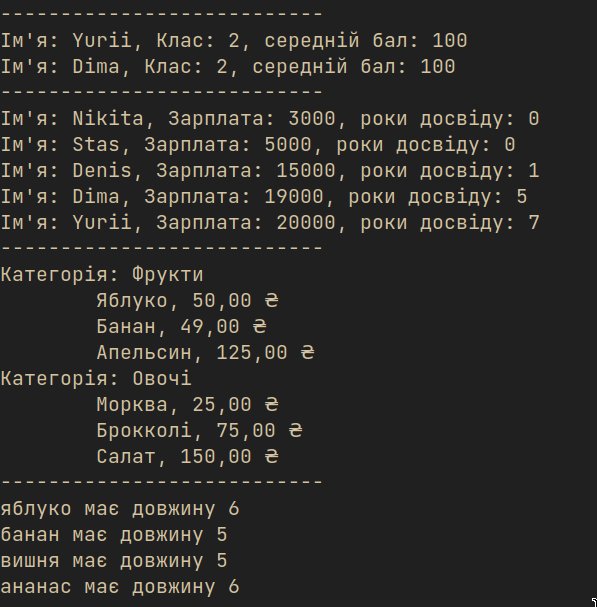
\includegraphics[width=0.8\textwidth]{img/2023-02-26-18-09-02.png}

\end{document}
